\chapter{Textual Search}\label{chap:text_search}

The model described in the previous chapter assigns each image $\bm{x}$ a vector $\bm{\hat{y}}$. In theory, it represents how likely each class is contained in the image. However, this representation is far from useful for a user. Therefore multiple techniques are used to ensure the model is a convenient yet powerful search tool even for novices.

\section{Supported Labels}
Our tool supports only a finite set of labels $L$ that are prompted by the interface when users form the query described in greater detail in Section \ref{chap:application_prototype}. It could be possible to construct a query given higher level description transformed by a task-specific set of neural language processing rules \cite{moumtzidou2017verge}, but this approach may mislead user if a searched high-level concept is not in an internal model. Thus a set $L_m$ is created containing labels corresponding to the image classes with their names, descriptions and hyponyms taken from WordNet \cite{WordNet}. We further utilize WordNet structure creating a new set $L_h$ of hypernyms of all labels in $L_m$. The final set of labels is then $L=L_m\cup L_h$. With hypernym--hyponym relation as a directed edge, $L$ can be viewed as a directed acyclic graph (DAG) where all vertices (i.e. labels) with no outgoing edges are in $L_m$ (however, there can be vertices in $L_m$ with outgoing edges).

\section{Query Formulation and Ranking}\label{sec:query_formulation_and_ranking}
The users are allowed to specify sets of supported labels $N_i \subseteq L$, wherein each set the labels are connected by logical \textsf{OR}, while the sets $N_i$ are connected by logical \textsf{AND}. For $k$ such sets, the user query $Q_u$ is then written as
\begin{equation}
	Q_u=\bigwedge\limits_{i=1}^k\left(\bigvee\limits_{\forall label_j\in N_i} label_j \right)\label{eq:cnf}
\end{equation}
and further in the text, for convenience, we use data representation of $Q_u$ defined as $\{N_i\}_{i=1}^k$ with the same meaning as in Equation \ref{eq:cnf}. If the query contains any hypernyms (labels with some outgoing edges in $L$), further preprocessing needs to be done. By default, every hypernym $h$ is substituted by a set of all labels in $L_m$ that are reachable from $h$ in DAG $L$. For hypernyms in $L_m$ (i.e. they correspond to a class recognized by the model), the substitution can be disabled. Finally, the preprocessed query $Q_p$ contains only labels from $L_m$ directly recognized by our model.

The ranking $r(\cdot)$ for each image $\bm{x}$, given preprocessed query $Q_p$ and model parametrized by $\bm{\theta}$, is calculated as 
\begin{equation}
r\left(\bm{x}; Q_p, \bm{\theta}\right)=\prod\limits_{\forall N_i \in Q_p}\left(
	\sum\limits_{\forall label_j\in N_i} \bm{\hat{y}}_{label_j}\cdot idf\left(label_j\right)
\right)\label{eq:text_rank}
\end{equation}
where $\bm{\hat{y}}=f\left(\bm{x}; \bm{\theta}\right)$  is model prediction on the image $\bm{x}$ and $\bm{\hat{y}}_{label_j}$ represents its relevance score of containing $label_j$ and $idf(\cdot)$ represents an inverse document frequency (IDF)~\cite{baeza1999modern}. Let us explain the underlying reasoning why to introduce IDF on an example: When a user searches \textit{a person in front of an excavator}, person keyword completely dominates the query since in the dataset there are thousand times as many persons as excavators. Standard IDF, however, uses the number of documents over the number of documents containing a given term which is unusable because softmax layer gives small nonzero values to almost all classes. We thus define inverse document frequency as
\begin{equation}
idf(label) = \log\left(
\frac{
\max\limits_{i\in labels} \sum_{\bm{x}}\hat{\bm{y}}_{i}
}{
\sum_{\bm{x}}\hat{\bm{y}}_{label}
} + 1\right)\label{eq:idf}
\end{equation}
where $\hat{\bm{y}}$ is the same as in Equation \ref{eq:text_rank}, therefore dependent on image $\bm{x}$. If we think of $\hat{\bm{y}}_i$ as a probability image $\bm{x}$ contains label $i$, the fraction in Equation \ref{eq:idf} can be viewed as how likely any given image contains the most common label in a collection over how likely it contains the searched label.

\section{Application Prototype}\label{chap:application_prototype}
This section discusses our user-friendly implementation of described approaches. Due to the project we are taking part in, the user interface is programmed in C\# language using the .NET framework and only focuses on an implementation of keyword search since the rest is developed jointly. Also note that model training, simulations, data annotation and other offline tasks presented in this work are programmed in Python and are available together with documentation on the attached CD (Attachment \ref{att:cd}). The user application can be logically divided into three parts described in the following sections: \textit{Main Window}, \textit{Keyword Model} and \textit{Suggestion Text Box}. Overview of the most important classes, their methods and interactions can be seen in Figure~\ref{fig:wpf_app}.

\begin{figure}[ht]
	\centering
	\begin{tikzpicture}[
box/.style={
	rectangle,
	draw=black,
	anchor=north west,
	text=black,
	text width=3.5cm,
	minimum height=0.7cm,
	font=\footnotesize,
	inner sep = 0.2cm,
	align=left,
	rectangle split, rectangle split parts=2,
	shading=axis,
	bottom color=bottomcol,top color=white,shading angle=45
}]
\definecolor{bottomcol}{RGB}{245,245,245}


\path[fill=yellow,opacity=0.05, draw=black] (0,-2.6) -- (-4.9,-2.6) -- (-4.9,-9.5) -- (9.3,-9.5) -- (9.3,-0.55) -- (4.15,-0.55) -- (4.15,-2.6) -- (3.9,-2.6);

\node[anchor=south west, font=\footnotesize, text=darkgray] at (-4.9,-9.5) {\textit{Suggestion Text Box}};

\node[box, rectangle split parts=3] (ksc) at (0,0) {
	{\centering \textbf{KWSearchControl} \par}
	\nodepart{second}
	{\scriptsize PUBLIC:}\\\quad
	\textit{Init() \\\quad
		Clear() \\\quad
		\Lightning\ KeywordChanged
	}\nodepart{third}
	{\scriptsize PRIVATE:}\\\quad
	\textit{QueryChanged()\\\quad
		SgnFilterChanged()\\\quad
		SgnNotNeeded()\\\quad
		GetSgnSubtree()
}};

% , below right=0cm and 1cm of ksc, anchor=south west
\node[box, below right=0cm and 1cm of ksc,anchor=south west] (stb) {
	{\centering \textbf{SgnTextBox} \par}
	\nodepart{second}
	{\scriptsize PUBLIC:}\\\quad
	\textit{\Lightning\ QueryChanged\\\quad
		\Lightning\ SgnFilterChanged\\\quad
		\Lightning\ GetSgnSubtree\\\quad
		\Lightning\ SgnNotNeeded \\\quad
		OnSgnResltReady() \\\quad
		OnShowSgnMsg()
}};
\node[box, below=0.5cm of ksc] (sp) {
	{\centering \textbf{SgnProvider} \par}
	\nodepart{second}
	{\scriptsize PUBLIC:}\\\quad
	\textit{GetSgn() \\\quad
		GetSgnAsync() \\\quad
		CancelSgn() \\\quad
		\Lightning\ SgnResultsReady\\\quad
		\Lightning\ ShowSgnMessage
}};

\node[box, below=0.5cm of stb] (sp) {
	{\centering \textbf{SgnPopup} \par}
	\nodepart{second}
	{\scriptsize PUBLIC:}\\\quad
	\textit{Open() \\\quad
		Close() \\\quad
		OnKeyDown() \\\quad
		\Lightning\ OnItemSelected\\\quad
		\Lightning\ OnItemExpanded
}};

\node[box] (lp) at (-4.4,-3.1) {
	{\centering \textbf{LabelProvider} \par}
	\nodepart{second}
	{\scriptsize PUBLIC:}\\\quad
	\textit{Labels
}};

\node[box, above left=0.5cm and 0.5cm of ksc] (mw) {
	{\centering \textbf{MainWindow} \par}
	\nodepart{second}
	{\scriptsize PRIVATE:}\\\quad
	\textit{KeywordChanged()\\\quad
		LoadFromConfig()
}};

\node[box, above right=0 and 0.5cm of mw, anchor=north west] (kmw) {
	{\centering \textbf{KWModelWrapper} \par}
	\nodepart{second}
	{\scriptsize PUBLIC:}\\\quad
	\textit{RankFrames()
}};

\node[box, above right=0 and 1cm of kmw, anchor=north west] (km) {
	{\centering \textbf{KWModel} \par}
	\nodepart{second}
	{\scriptsize PUBLIC:}$\ $\textit{RankFrames()
}};

\draw[o->, dotted] (0.35,-2.2) -- (-4.6,-2.2) -- (-4.6,1.35) -- (-4.05,1.35);

\draw[-stealth,shorten >=0.05cm, shorten <=0.05cm] (-0.5,1.6) -- (0,1.6);

\draw[-stealth,shorten >=0.05cm, shorten <=0.05cm] (-0.5,0.5) -- (0,0);

\draw[-stealth,shorten >=0.2cm, shorten <=0.2cm] (3.9,2) -- (4.9,2);
\draw[-stealth,shorten >=0.2cm, shorten <=0.2cm] (3.9,1.8) -- (4.9,1.8);
\draw[-stealth,shorten >=0.2cm, shorten <=0.2cm] (3.9,2.2) -- (4.9,2.2);


\node[cylinder,fill=bottomcol, shape border rotate=90, aspect=1, inner sep=2pt, minimum width=1cm, draw, anchor=north] at (-2.45,-6) {};
\node[cylinder,fill=bottomcol, shape border rotate=90, aspect=1, inner sep=2pt, minimum width=1cm, draw, anchor=north] at (-2.45,-5.75) {};
\node[cylinder,fill=bottomcol, shape border rotate=90, aspect=1, inner sep=2pt, minimum width=1cm, draw, anchor=north] at (-2.45,-5.5) {};
\node[font=\footnotesize] at (-2.45,-6.6) {\textit{.label}};
\draw[-stealth,shorten >=0.1cm, shorten <=0.1cm] (-2.45,-4.8) -- (-2.45,-5.5);


\node[cylinder,fill=bottomcol, shape border rotate=90, aspect=1, inner sep=2pt, minimum width=1cm, draw, anchor=north] at (-2.45,-0.7) {};
\node[cylinder,fill=bottomcol, shape border rotate=90, aspect=1, inner sep=2pt, minimum width=1cm, draw, anchor=north] at (-2.45,-0.45) {};
\node[cylinder,fill=bottomcol, shape border rotate=90, aspect=1, inner sep=2pt, minimum width=1cm, draw, anchor=north] at (-2.45,-0.2) {};
\node[font=\footnotesize] at (-2.45,-1.3) {\textit{images}};
\draw[-stealth,shorten >=0.1cm, shorten <=0.1cm] (-2.45,0.5) -- (-2.45,-0.2);


\node[cylinder,fill=bottomcol, shape border rotate=90, aspect=1, inner sep=2pt, minimum width=1cm, draw, anchor=north] at (6.0,0.3) {};
\node[cylinder,fill=bottomcol, shape border rotate=90, aspect=1, inner sep=2pt, minimum width=1cm, draw, anchor=north] at (6.0,0.55) {};
\node[cylinder,fill=bottomcol, shape border rotate=90, aspect=1, inner sep=2pt, minimum width=1cm, draw, anchor=north] at (6.0,0.8) {};
\node[font=\footnotesize] at (6.0,-0.3) {\textit{.keyword}};
\draw[-stealth,shorten >=0.1cm, shorten <=0.1cm] (6.0,1.275) -- (6.0,0.8);

\node[cylinder,fill=bottomcol, shape border rotate=90, aspect=1, inner sep=2pt, minimum width=1cm, draw, anchor=north] at (7.7,0.3) {};
\node[cylinder,fill=bottomcol, shape border rotate=90, aspect=1, inner sep=2pt, minimum width=1cm, draw, anchor=north] at (7.7,0.55) {};
\node[cylinder,fill=bottomcol, shape border rotate=90, aspect=1, inner sep=2pt, minimum width=1cm, draw, anchor=north] at (7.7,0.8) {};
\node[font=\footnotesize] at (7.7,-0.3) {\textit{.idf}};
\draw[-stealth,shorten >=0.1cm, shorten <=0.1cm] (7.7,1.275) -- (7.7,0.8);


\draw[o->, dotted] (5.25,-2.5) -- (4.25,-2.5) -- (4.25,-3.35) -- (3.7,-3.35);
\draw[o->, dotted] (5.25,-2.9) -- (4.35,-2.9) -- (4.35,-3.75) -- (3.7,-3.75);
\draw[o->, dotted] (5.25,-3.3) -- (4.45,-3.3) -- (4.45,-4.2) -- (3.7,-4.2);
\draw[o->, dotted] (5.25,-3.75) -- (4.55,-3.75) -- (4.55,-4.6) -- (3.7,-4.6);

\draw[o->, dotted] (3.7,-8.2) -- (4.65,-8.2) -- (4.65,-4.15) -- (5.25,-4.15);
\draw[o->, dotted] (3.7,-8.65) -- (4.75,-8.65) -- (4.75,-4.6) -- (5.25,-4.6);

\draw[o->, dotted, shorten >=0.2cm] (8.6,-8.2) -- (9,-8.2) -- (9,-5.4) -- (8.8,-5);
\draw[o->, dotted, shorten >=0.2cm] (8.6,-8.65) -- (9.1,-8.65) -- (9.1,-5.1) -- (8.8,-5);

\draw[-stealth,shorten >=0.05cm, shorten <=0.05cm] (1.95,-5) -- (1.95,-5.5);
\draw[-stealth,shorten >=0.05cm, shorten <=0.05cm] (1.75,-5) -- (1.75,-5.5);
\draw[-stealth,shorten >=0.05cm, shorten <=0.05cm] (2.15,-5) -- (2.15,-5.5);

\draw[-stealth,shorten >=0.05cm, shorten <=0.05cm] (0,-4) -- (-.5,-4);
\draw[-stealth,shorten >=0.05cm, shorten <=0.05cm] (0,-4.2) -- (-.5,-4.2);
\draw[-stealth,shorten >=0.05cm, shorten <=0.05cm] (0,-3.8) -- (-.5,-3.8);

\draw[-stealth,shorten >=0.05cm, shorten <=0.05cm] (0,-5.5) -- (-.5,-4.8);

\draw[-stealth,shorten >=0.05cm, shorten <=0.05cm] (6.85,-5) -- (6.85,-5.5);
\draw[-stealth,shorten >=0.05cm, shorten <=0.05cm] (6.65,-5) -- (6.65,-5.5);
\draw[-stealth,shorten >=0.05cm, shorten <=0.05cm] (7.05,-5) -- (7.05,-5.5);
\end{tikzpicture}

	
	\caption[Application prototype structure]{Application prototype structure. A solid arrow represents a reference to a class instance. Multiple arrows denote, that reference to more instances is possible. A dotted arrow represents a reference to a function. Interaction with external data files is denoted by a database icon.}
	\label{fig:wpf_app}
\end{figure}

\subsection{Main Window}
The Main Window class is used as an entry point for the application defining its user interface and connecting the text box to the retrieval model. It is also responsible for correctly initializing all the components with appropriate external data files defined in a configuration file. Further, since the application is only a demo, the class loads and displays images to a user based on a model's ranking.


\subsection{Keyword Model}
Keyword model implements the ranking algorithm as described in the section above. An inverted index is utilized for fast query retrieval. As the creation of the index is the most demanding operation due to the image annotation by DCNN, it is created once in the preprocessing phase. The neural network assigns each image $\bm{x}^{(i)}$ set of labels with its score $\{(label_j,\hat{\bm{y}}_{label_j})\given{\hat{\bm{y}}=f(\bm{x}^{(i)};\bm{\theta})},\  {label_j\in L_m}\}$. Further, labels with a score lower than $0.001$ are discarded without loss of model's quality as discussed in Chapter~\ref{chap:evaluation}. The inverted index then contains for each label $j\in L_m$ list of tuples $(i, \hat{\bm{y}}_{label_j})$ -- image id and assigned score. The file also incorporates label-to-offset map that enables fast seek instructions to individual label lists.

During application startup, only the label-to-offset map is loaded into RAM. Lists corresponding to the given labels are copied into the memory only when the model is queried by a user. For small datasets, the overhead is negligible since there are more I/O intensive operations such as image rendering, etc. For large collections, the slowdown can be noticed if a compound query is created yet this approach saves space in RAM that can be used by other more memory demanding models such as similarity model. Also note, that the most labels are not used each time the application is run since only a handful of keywords are used per each target image. To mitigate the possible slowdown the model uses two caches. The bigger one stores already loaded labels avoiding virtually any repetitive label read during regular usage. The smaller one stores clauses (i.e. $\bigvee_i label_i$) enabling faster retrieval of repeated or more complex queries. The application also supports multiple keyword sources, therefore, Keyword Model Wrapper is used to redirect model calls to appropriate models.

\begin{figure}[ht]
	\centering
	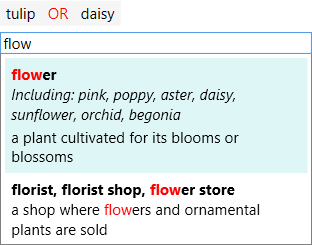
\includegraphics[scale=0.5]{img/keyword-textbox.png}
	
	\caption[Keyword search interface]{Keyword search interface. When selecting the \textit{flower} label, hyponyms \textit{pink}, \textit{poppy}, etc. will also be searched. To select only \textit{flower}, a user can hold the control key while pressing the enter. If the label is expanded by pressing the right key, the user can also select only individual flowers.}
	\label{fig:keyword-textbox}
\end{figure}

\subsection{Suggestion Text Box}
The suggestion-providing text box is comprised of multiple classes encapsulated by Keyword Search Control class enabling effortless integration to any existing application. If text box's content changes, a handler in Keyword Search Control selects Suggestion Provider belonging to the currently selected keyword source. The provider asynchronously searches all labels $l\in L$ and hands over the results to the text box when completed. Suggestion Popup is then populated with the results, displaying them to a user. If any suggestion is selected to update the query, Keyword Search Control passes a list of selected labels to a registered handler responsible for a query ranking.

The text box accepts only the labels $L$, however, full-text search over their WordNet names and descriptions is performed using Aho--Corasick string search algorithm. This way, a user gets suggestions even if the desired label is not present and thus can select any similar label based on its description or quickly see that the query needs to be formulated differently. As user types, the suggestions are presented with the searched phrase highlighted (see Figure \ref{fig:keyword-textbox}). The labels are distinguished by color. Red labels are the added WordNet hypernyms $L_h$, green and gray labels represent basic 1150 labels $L_m$. The green labels represent hypernyms for gray labels. The suggestions are browsed by up and down keys, while the selection of keyword is done only by enter. We find mouse control unnecessary since interaction via keyboard is faster, but we may include more intuitional and user-friendly mouse control for novices as well. When a user browses to a hypernym, the right key can be used to expand the hypernym, following the WordNet structure. When a label is selected, it appears on the top panel, connected by logical \textsf{OR} with previously selected labels. Logical relation between the labels can be changed to \textsf{AND} and back by left mouse click, clicking on the labels themselves removes them from the query.

\section{Other Retrieval Models}
Our work is part of a bigger project focused on video retrieval with a goal of creating a tool that provides a user with a powerful means to interactively search his video collection. In this section, we therefore summarize our tool's other retrieval models and model fusion used for Lifelog Search Challenge (LSC) workshop at ICMR2018~\cite{LokocLSC} and for Video Browser Showdown (VBS) competition at MMM2018~\cite{lokovc2018revisiting}.

Mainly for visual KIS tasks, our tool features easy-to-use canvas for color sketches. Every sketch is represented as a set $Q_c = \{\left(q_i, r_i, t_i\right)\}^k_{i=1}$ of $k$ color points where $q_i\in\R^3$ is color in CIE Lab color space, $r_i$ represents region where the given color shall be located and $t_i\in \{\mathrm{ALL},\mathrm{ANY}\}$ specifies whether ALL or just ANY of the pixels in the region should be considered. The ranking $c(\cdot)$ of an image $\bm{x}$ is then computed as
\begin{equation}
c\left(\bm{x}; Q_c\right) =-\left(\sum\limits_{\substack{\forall \left(q_i,r_i,t_i\right) \in Q_c\\t_i=\mathrm{ANY}}} \min\limits_{p\in\bm{x}\,\mathrm{in}\,r_i}L_2\left(q_i, p\right)+\sum\limits_{\substack{\forall \left(q_i,r_i,t_i\right) \in Q_c\\t_i=\mathrm{ALL}}} \mathop{\mathrm{avg}}\limits_{p\in\bm{x}\,\mathrm{in}\,r_i}L_2\left(q_i, p\right)\right)
\end{equation}
where $p\in\bm{x}\ \mathrm{in}\ r_i$ represents all pixels of image $\bm{x}$ in specified region $r_i$. Due to performance reasons, each image in the database is represented only as $20\times 15$ color points or `pixels'. Our user interface also currently supports regions in the shape of ellipses only. If a keyword or color-sketch search is not successful or a user wants to simply browse similar images, our tool utilizes deep features from GoogLeNet~\cite{szegedy2015going} after the last average pooling layer for retrieval of semantically similar images. Rank of an image given a query example is the cosine similarity between their deep feature vectors.


All the retrieval models provide a relevance score function inducing a similarity based ordering of all database objects with respect to a given query. Even though our tool supports multiple query modalities at once by normalizing the ranking of each modality to the interval $[0, 1]$ and then summing them up, combining multiple models can be tricky. This is because each model has a different distribution of rank values, e.g. similarity ranking assigns to most of the database rank between $0.6$ and $0.85$ whereas in keyword ranking almost all images are assigned rank smaller than~$10^{-2}$. However, our tool enables us to use other models as filters where their thresholds can be dynamically set for each model interdependently. Such an approach proved to be much more useful than sorting joined ranking from multiple models.

